\documentclass{beamer}

%% Use package -----------------------------------------------------------------

\usepackage[T1]{fontenc}
\usepackage[utf8]{inputenc}
\usepackage{lmodern}
\usepackage{graphicx}
\usepackage[absolute,overlay]{textpos}
\usepackage{multicol}
\usepackage{listings}

%% Beamer customization---------------------------------------------------------

\usepackage{xcolor}
\usetheme{Warsaw}

%% Themes
% Outer themes
\useoutertheme{shadow}
% Rounded boxes and shadows
\useinnertheme[shadow=true]{rounded}
% Solid \item symbols
\useinnertheme{circles}

%% Custom colors
\definecolor{rltgreen}{rgb}{0,0.5,0}
\definecolor{pasteur}{RGB}{0,90,154}
\setbeamerfont{block title}{size={}}
\setbeamercolor{structure}{fg=pasteur}
\setbeamercolor{item}{fg=pasteur}

%Color of title
\setbeamertemplate{frametitle}
{
    \nointerlineskip
    \begin{beamercolorbox}[sep=0.3cm,ht=1.8em,wd=\paperwidth]{frametitle}
        \vbox{}\vskip-2ex%
        \strut\insertframetitle\strut
        \vskip-0.8ex%
    \end{beamercolorbox}
}
% Hide navigation symbols
\setbeamertemplate{navigation symbols}{}

%% Title block
\setbeamercolor*{title}{use=structure,fg=white,bg=pasteur}

%% Bottom infolines
\setbeamertemplate{footline}
{
  \leavevmode%
  \hbox{%
  \begin{beamercolorbox}[wd=.3\paperwidth,ht=2.25ex,dp=1ex,center]{author in head/foot}%
    \usebeamerfont{author in head/foot}\insertshortauthor
  \end{beamercolorbox}%
  \begin{beamercolorbox}[wd=.7\paperwidth,ht=2.25ex,dp=1ex,center]{title in head/foot}%
    \usebeamerfont{title in head/foot}\insertshorttitle\hspace*{3em}
    \insertframenumber{} / \inserttotalframenumber\hspace*{1ex}
  \end{beamercolorbox}}%
  \vskip0pt%
}
\makeatletter

%% Top infolines
\setbeamertemplate{headline}{%
\leavevmode%
  \hbox{%
    \begin{beamercolorbox}[wd=\paperwidth,ht=2.5ex,dp=1.125ex]{palette quaternary}%
    \insertsectionnavigationhorizontal{\paperwidth}{}{\hskip0pt plus1filll}
    \end{beamercolorbox}%
  }
}

%% Define Snakemake ------------------------------------------------------------

\definecolor{eclipseBlue}{RGB}{42,0.0,255}
\definecolor{eclipseGreen}{RGB}{63,127,95}
\definecolor{eclipsePurple}{RGB}{127,0,85}

\lstset{language=Python}
\lstset{
    basicstyle=\tiny\ttfamily,
    morekeywords={rule, output, shell, params, run, configfile, temp, threads, log},
    showstringspaces=false,
    commentstyle=\color{eclipseGreen}, % style of comments
    keywordstyle=\color{eclipsePurple}, % style of keywords
    stringstyle=\color{eclipseBlue}, % style of strings
}


%% Set up title ----------------------------------------------------------------

\title{Snakemake Presentation}
\author[D.Desvillechabrol \& T.Cokelaer]{Dimitri Desvillechabrol and Thomas Cokelaer}
\institute{Institut Pasteur}
\date{March 22 2016}

\begin{document}

%% Title slide -----------------------------------------------------------------

\begin{frame}[plain]
    \titlepage
    \begin{textblock*}{5cm}(4.5cm,0.3cm)
        
\includegraphics[scale=0.09]{../images/Institut_Pasteur.png}
    \end{textblock*}
\end{frame}

%% Slides ----------------------------------------------------------------------

\section{Introduction}
% Introduction to how it is useful
%% git philosophy
%% Useful for bioinformatics services
%% Useful for software development
%% Differences with svn?

\begin{frame}
\frametitle{philosophy}


\end{frame}


\section{Basic git}
% Basic philosophy and usage
\graphicspath{{images/}}


%\begin{frame}[fragile]{The central and local repository}
%  
\includegraphics[height=0.9\textheight, width=\textwidth]{images/distributed}
%\end{frame}


\begin{frame}[fragile]{Configuration}
	\begin{lstlisting}
$ git config --global user.name "First Last"
$ git config --global user.email "email@example.com"
$ git config --global color.diff "auto"
$ git config --global color.status "auto"
$ git config --global color.branch "auto"
	\end{lstlisting}
\end{frame}

\setbeamercovered{transparent=0}

\begin{frame}[fragile]{Create/Clone a repository}
	\begin{columns}
		\begin{column}{0.6\textwidth}
			\begin{lstlisting}
$ # Create a local repository in the current folder
$ git init |\pause|

$ # or clone a remote repository
$ git clone https://github.com/C3BI-pasteur-fr/tutorials.git
			\end{lstlisting}
		\end{column}
		\begin{column}{0.4\textwidth}
			\begin{center}
				\only<1> {
					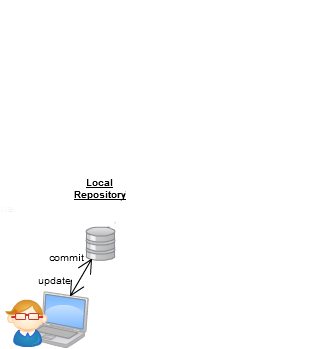
\includegraphics[width=0.9\textwidth]{init.png}
				}\only<2> {
					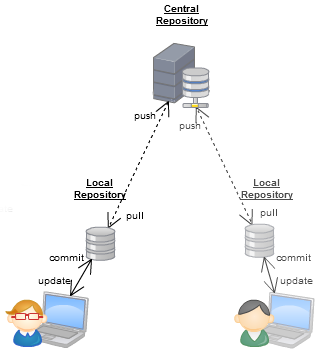
\includegraphics[width=0.9\textwidth]{clone.png}
				}
			\end{center}
		\end{column}
	\end{columns}
\end{frame}


\begin{frame}[fragile]{First steps}
	\begin{columns}
		\begin{column}{0.6\textwidth}
			\begin{lstlisting}
|\pause|
$ # Create a file
$ touch README.txt  |\pause|

$ # Add files to index (to be committed)
$ git add README.txt |\pause|

$ # Look at the current index state 
$ git status
On branch master

Initial commit

Changes to be committed:
  (use "git rm --cached <file>..." to unstage)

	new file:   README.txt |\pause|

$ # Commit (to our local repository!)
$ git commit README.txt -m "Added README file"
[master (root-commit) b84669e] Added README file
 1 file changed, 0 insertions(+), 0 deletions(-)
 create mode 100644 README.txt |\pause|
 
$ # Push to the remote server
$ git push 
			\end{lstlisting}
		\end{column}
		\begin{column}{0.4\textwidth}
			\begin{center}
				\only<1> {
					
\includegraphics[width=0.9\textwidth]{empty.png}
				}\only<2-4> {
					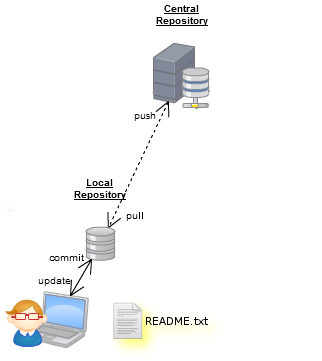
\includegraphics[width=0.9\textwidth]{touch.png}
				}\only<5> {
					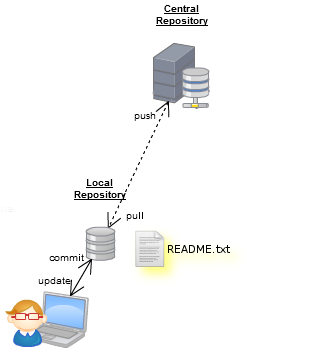
\includegraphics[width=0.9\textwidth]{commit.png}
				}\only<6> {
					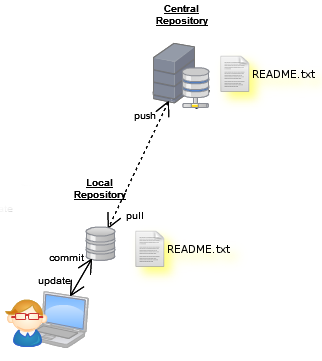
\includegraphics[width=0.9\textwidth]{push.png}
				}
			\end{center}
		\end{column}
	\end{columns}
\end{frame}


%\begin{frame}
%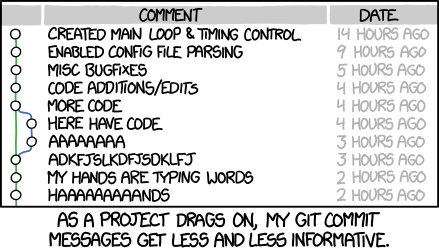
\includegraphics[height=0.9\textheight, width=\textwidth]{images/git_commit}
%\end{frame}


\begin{frame}{Everything is a branch!}
	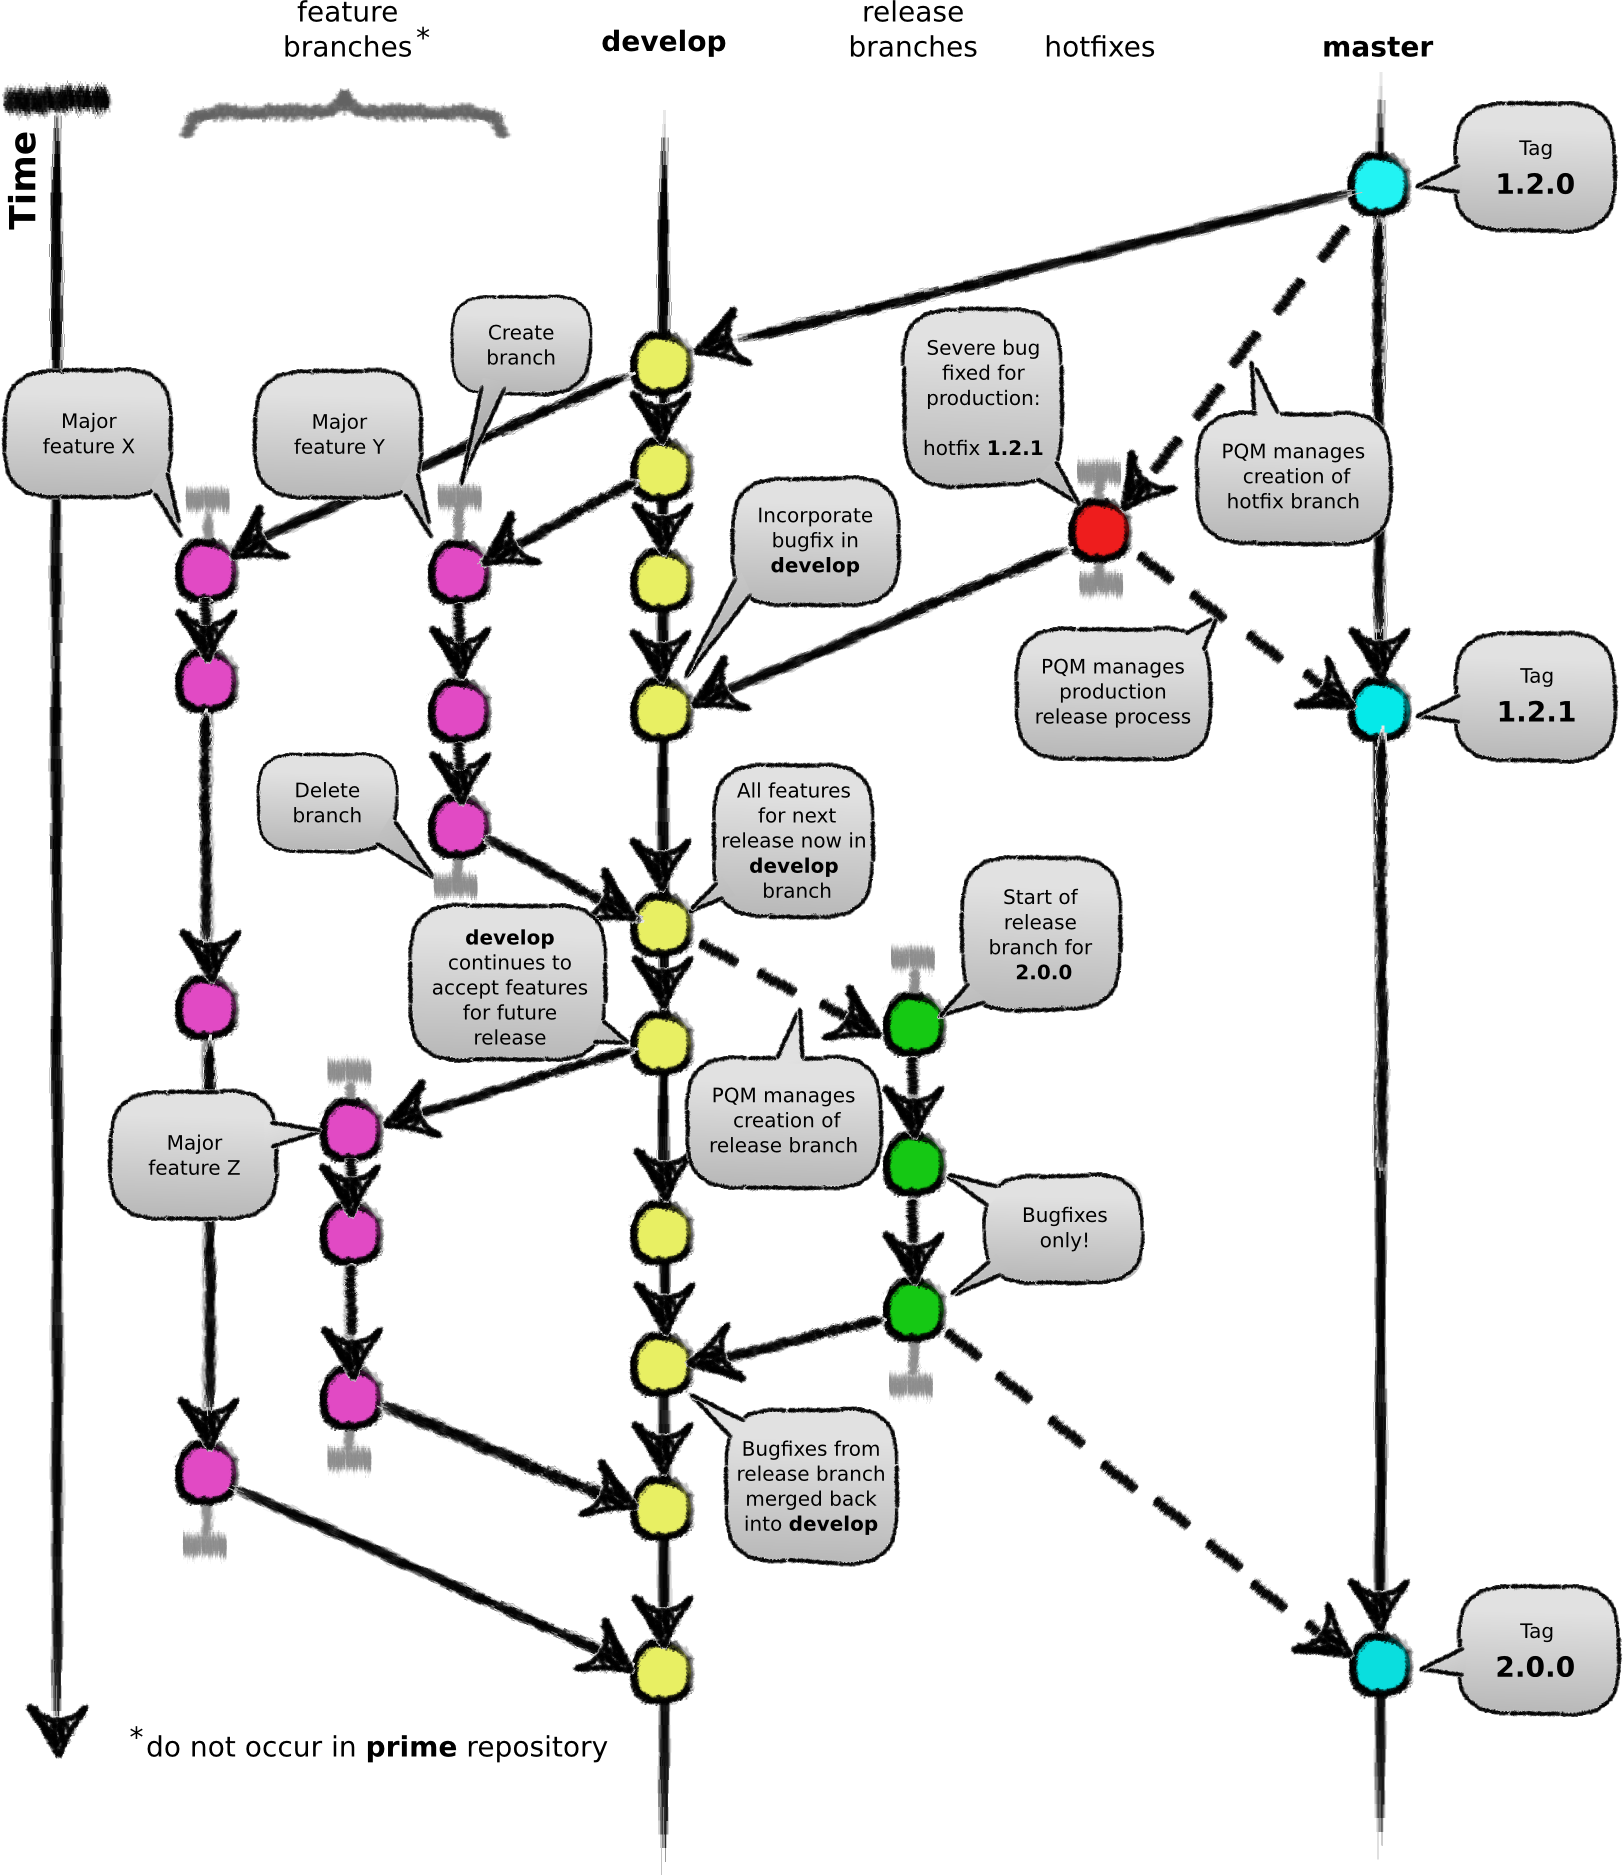
\includegraphics[height=0.9\textheight, width=\textwidth]{gitflow}
\end{frame}

\subsection{One-user case}

\begin{frame}[fragile]{Implement a new feature/Fix a bug}
\begin{columns}
	\begin{column}{0.6\textwidth}
	\small
	\begin{enumerate}
		\item Create a new branch
		\item Implement a new feature/Fix a bug
		\begin{enumerate}
			\tiny
			\item Step 1 towards new feature/bug fix
			\item Commit
			\item Step 2 towards new feature/bug fix
			\item Commit
			\item \ldots
		\end{enumerate}
		\item Update the master
		\item Delete this branch 
	\end{enumerate}
	\end{column}
	\begin{column}{0.4\textwidth}
		\begin{center}
			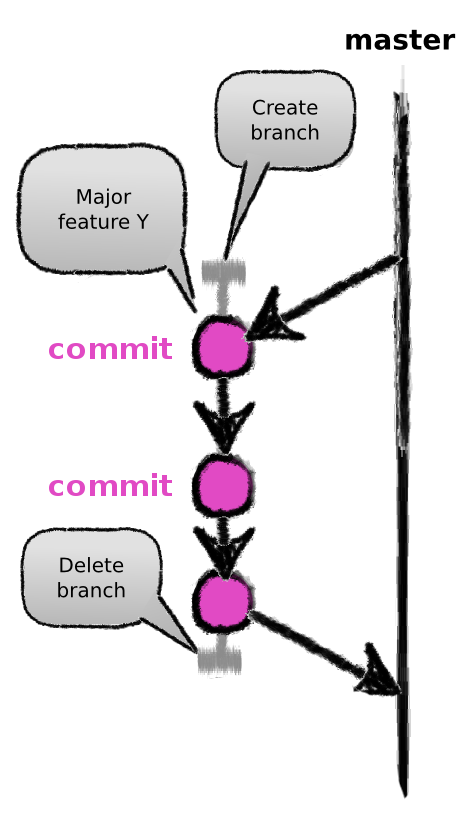
\includegraphics[width=0.9\textwidth]{branch.png}
		\end{center}
	\end{column}
\end{columns}
\end{frame}


\begin{frame}[fragile]{Step 1. Create a new branch locally}
\begin{columns}
	\begin{column}{0.6\textwidth}
	\begin{lstlisting}
$ # Which branches do we have?
$ git branch -a
* master
remotes/origin/HEAD -> origin/master
remotes/origin/master
remotes/origin/services |\pause|

$ # Create a branch for our feature/bug fix...
$ git branch feature
$ # ... and switch to this branch
$ git checkout feature 
Switched to a new branch "feature" |\pause|

$ # or create + switch in one command
$ git checkout -b feature 
Switched to a new branch "feature"
  	\end{lstlisting}
  	\end{column}
	\begin{column}{0.4\textwidth}
		\begin{center}
			\only<1> {
				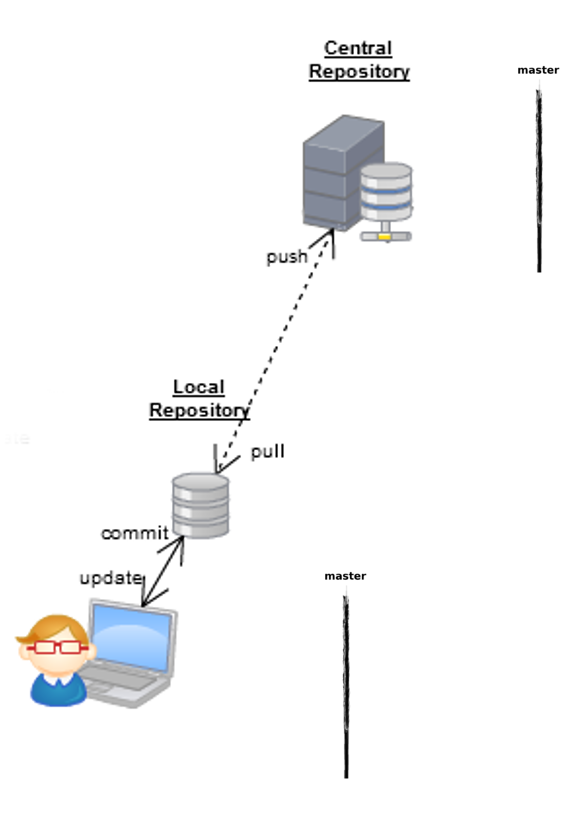
\includegraphics[width=0.9\textwidth]{branch_a.png}
			} \only<2-> {
				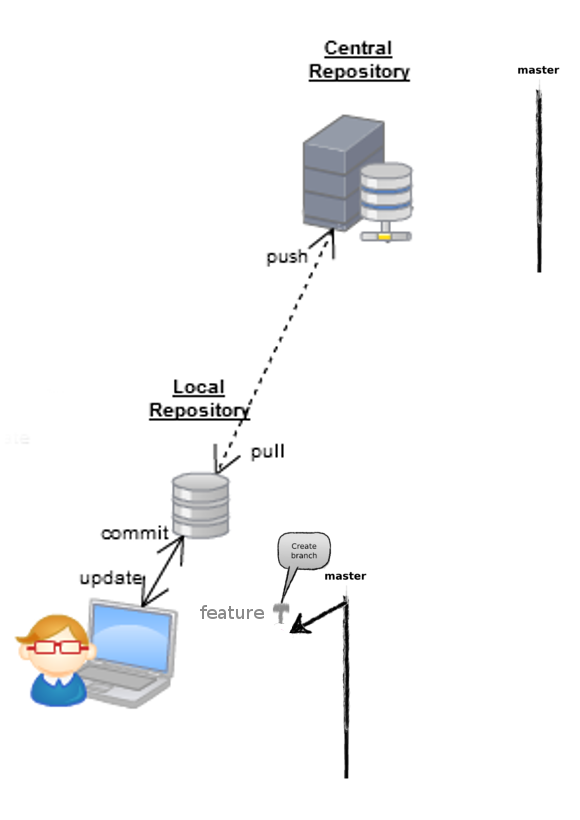
\includegraphics[width=0.9\textwidth]{branch_created.png}
			}
		\end{center}
	\end{column}
\end{columns}
\end{frame}


\begin{frame}[fragile]{Step 2. Implement a new feature/Fix a bug}
\begin{columns}
	\begin{column}{0.6\textwidth}
	\begin{lstlisting}
$ # Add files to index (to-be-committed)
$ git add main.py __init__.py |\pause|

$ # Look at current index state
$ git status
On branch feature
Changes to be committed:
  (use "git reset HEAD <file>..." to unstage)

	modified:   main.py

Changes not staged for commit:
  (use "git add <file>..." to update what will be committed)
  (use "git checkout -- <file>..." 
	to discard changes in working directory)

	modified:   __init__.py |\pause|

$ # Commit (to our local repository!)
$ git commit -m "Fixed TSS positions on - strand"
[feature fd07832] Fixed TSS positions on - strand
 1 file changed, 1 insertion(+) 
  	\end{lstlisting}
  	\end{column}
	\begin{column}{0.4\textwidth}
		\begin{center}
			\only<1-2> {
				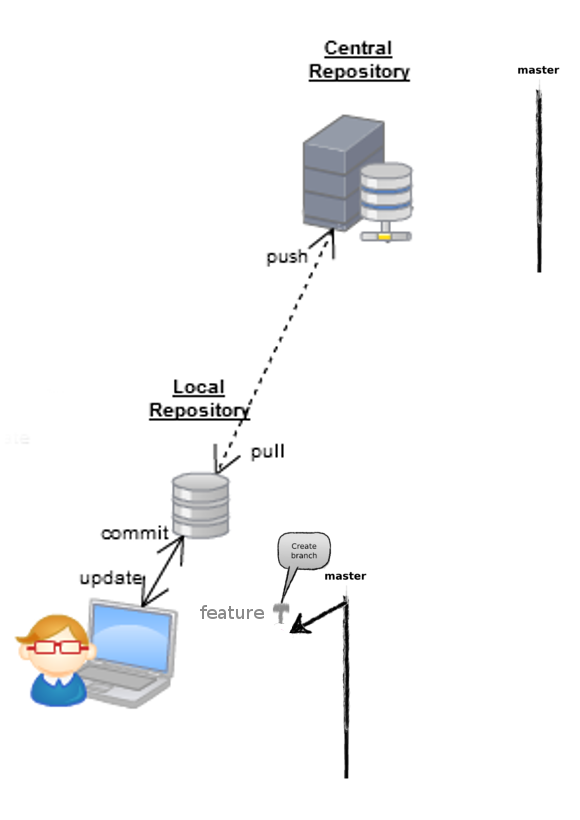
\includegraphics[width=0.9\textwidth]{branch_created.png}
			} \only<3-> {
				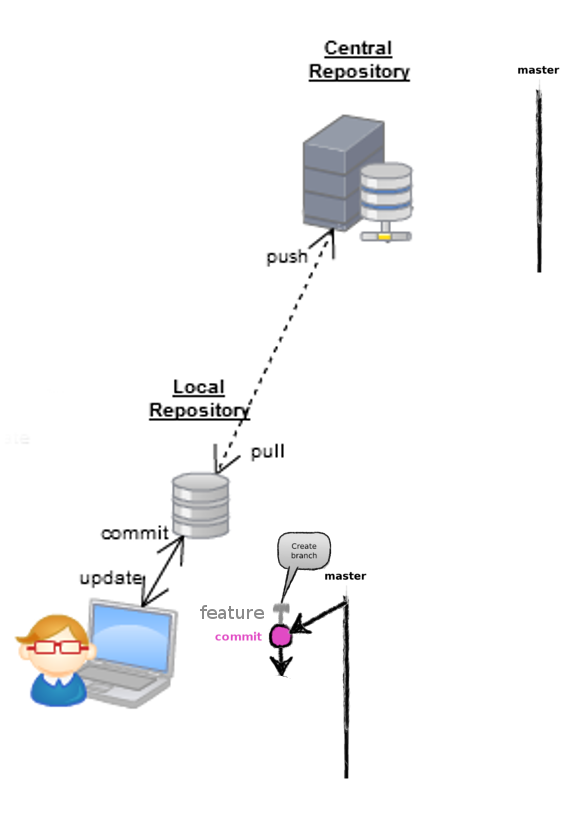
\includegraphics[width=0.9\textwidth]{branch_commit.png}
			}
		\end{center}
	\end{column}
\end{columns}
\end{frame}


\begin{frame}[fragile]{Steps 3-4. Update the master and delete the branch}
\begin{columns}
	\begin{column}{0.6\textwidth}
  	\begin{lstlisting}
# Switch to master
$ git checkout master
Switched to branch 'master' |\pause|

$ # Reapply our commits on the master branch
$ git rebase feature
First, rewinding head to replay your work on top of it...
Fast-forwarded master to feature. |\pause|

$ # Delete local branch
$ git branch -d feature
Deleted branch feature (was fd86490). |\pause|

$ # Push changes to the remote server (origin)
$ git push origin master
	\end{lstlisting}
	\end{column}
	\begin{column}{0.4\textwidth}
		\begin{center}
			\only<1> {
				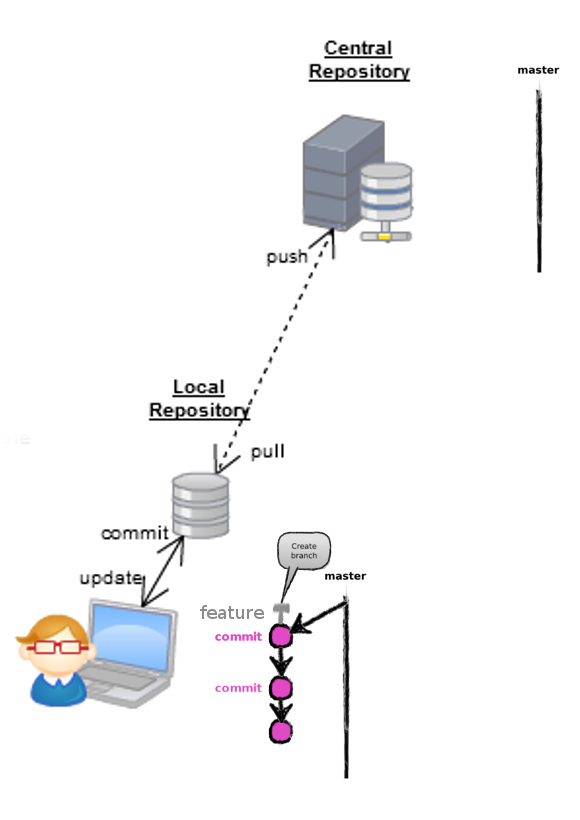
\includegraphics[width=0.9\textwidth]{branch_committed.png}
			}\only<2> {
				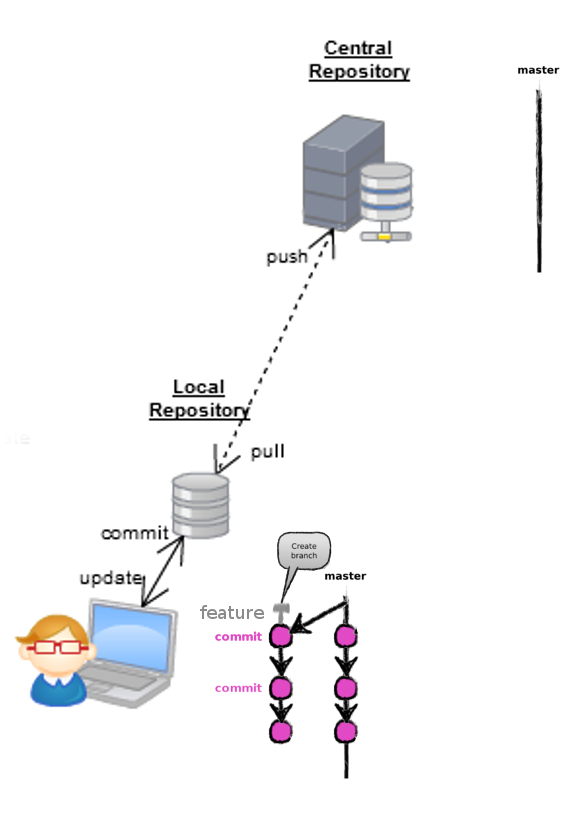
\includegraphics[width=0.9\textwidth]{branch_rebase.png}
			}\only<3> {
				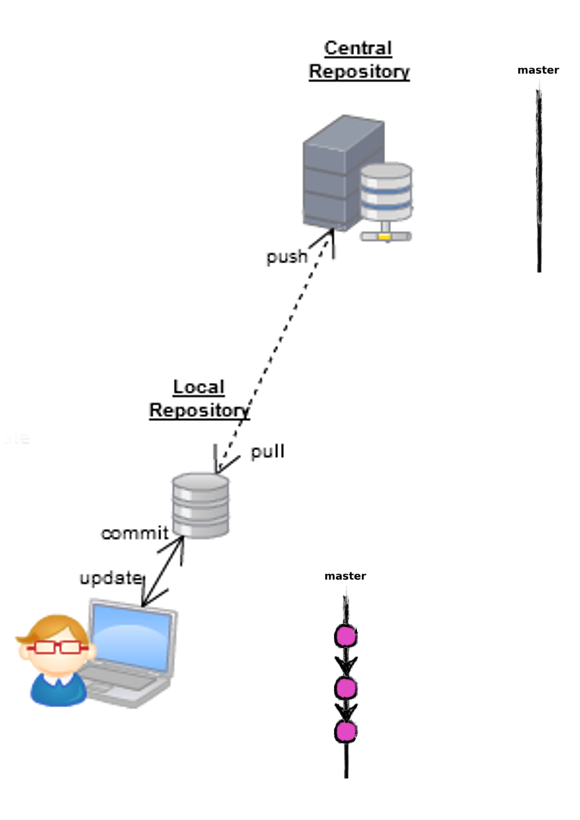
\includegraphics[width=0.9\textwidth]{branch_delete.png}
			}\only<4> {
				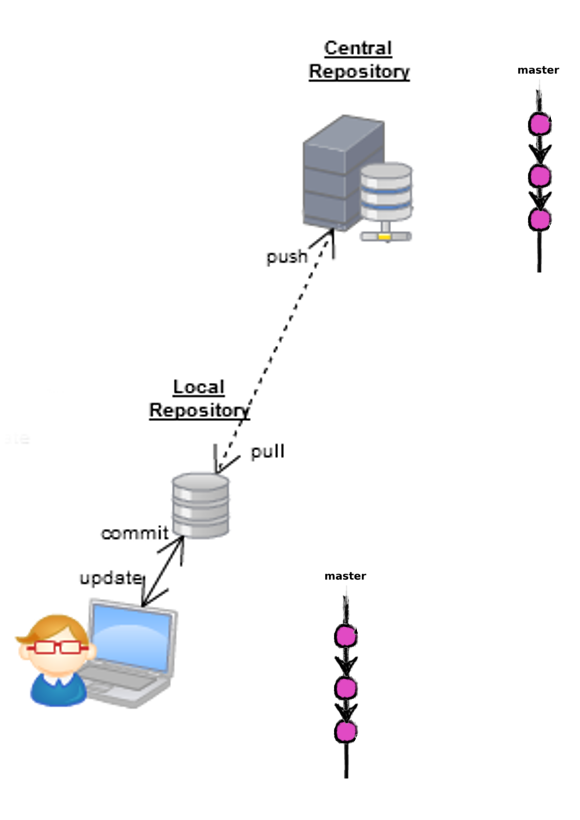
\includegraphics[width=0.9\textwidth]{branch_pushed.png}
			}
		\end{center}
	\end{column}
\end{columns}
\end{frame}

\setbeamercovered{transparent=30}

\begin{frame}[fragile]{The scenario we've just seen}

\subsection{Multiuser case}
\begin{columns}
\begin{column}{0.6\textwidth}
	\tiny
	\begin{enumerate}
		\item<2> Created a new branch \textbf{locally}
		\item<3-4> Implemented a new feature/bug fix
		\begin{enumerate}
			\tiny
			\item<3> Step 1 towards new feature
			\item<3> Commit
			\item<4> Step 2 towards bug fix
			\item<4> Commit
			\item<4> \ldots
		\end{enumerate}
		\item<5> \textbf{Reapplied} the commits from this branch on the master \textbf{locally}
		\item<6> Deleted this branch \textbf{locally} (it never existed elsewhere)
		\item<7> Pushed changes to the remote server (origin)
	\end{enumerate}
\end{column}
\begin{column}{0.4\textwidth}
	\begin{center}
			\only<1> {
				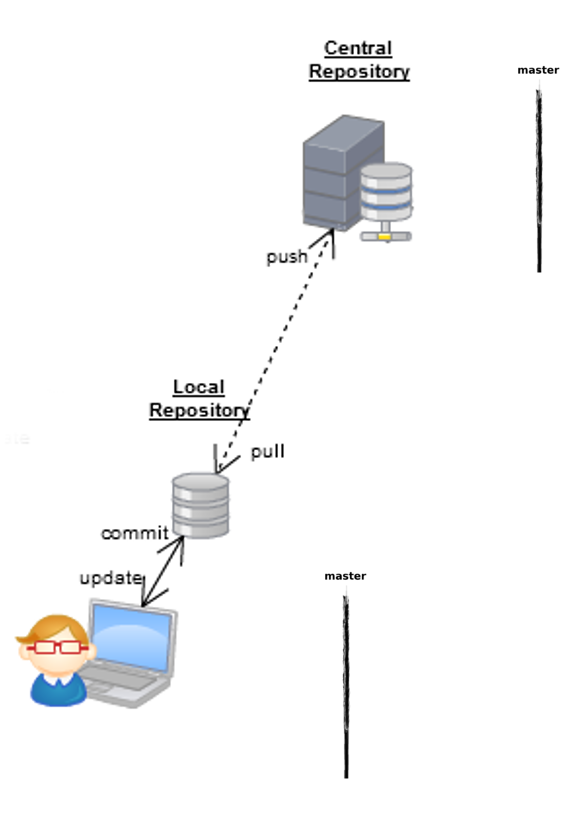
\includegraphics[width=0.9\textwidth]{branch_a.png}
			}\only<2> {
				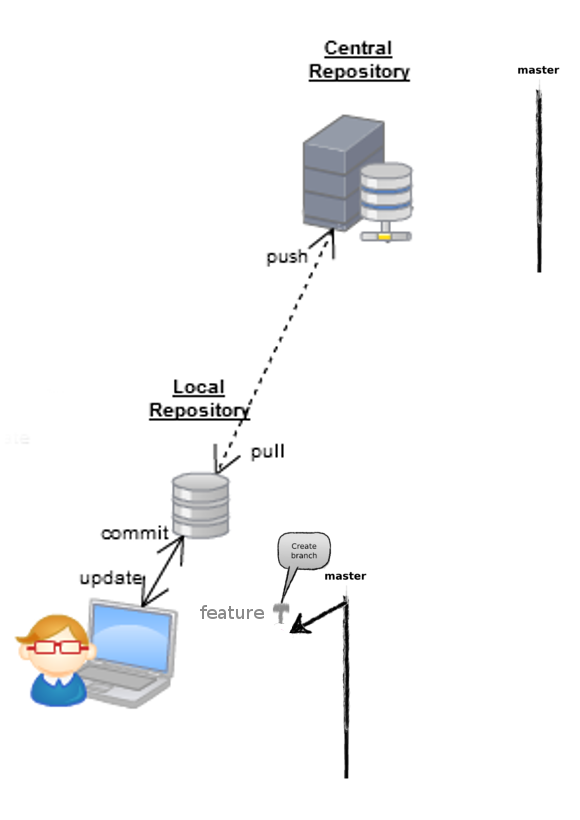
\includegraphics[width=0.9\textwidth]{branch_created.png}
			}\only<3> {
				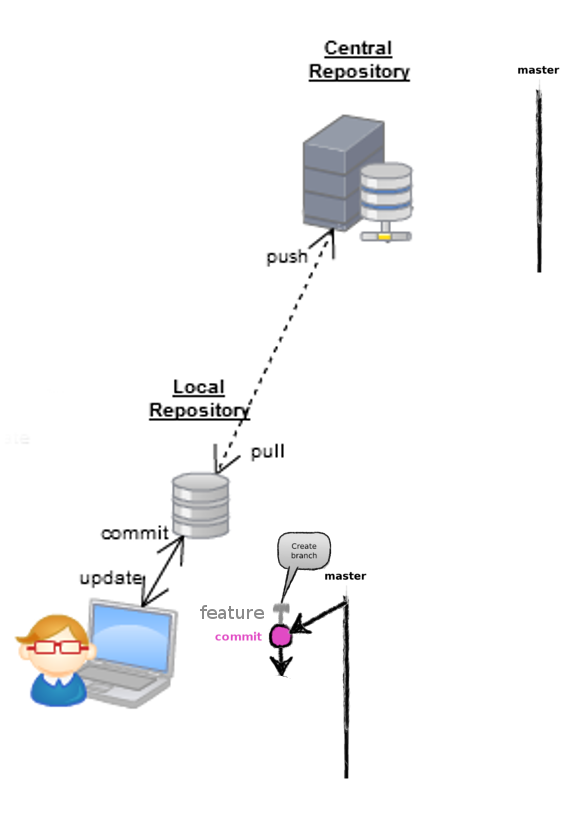
\includegraphics[width=0.9\textwidth]{branch_commit.png}
			}\only<4> {
				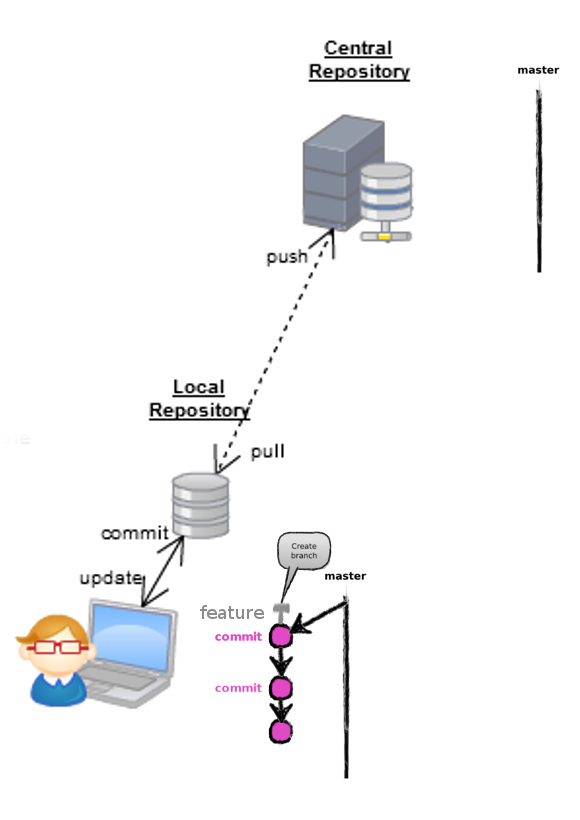
\includegraphics[width=0.9\textwidth]{branch_committed.png}
			}\only<5> {
				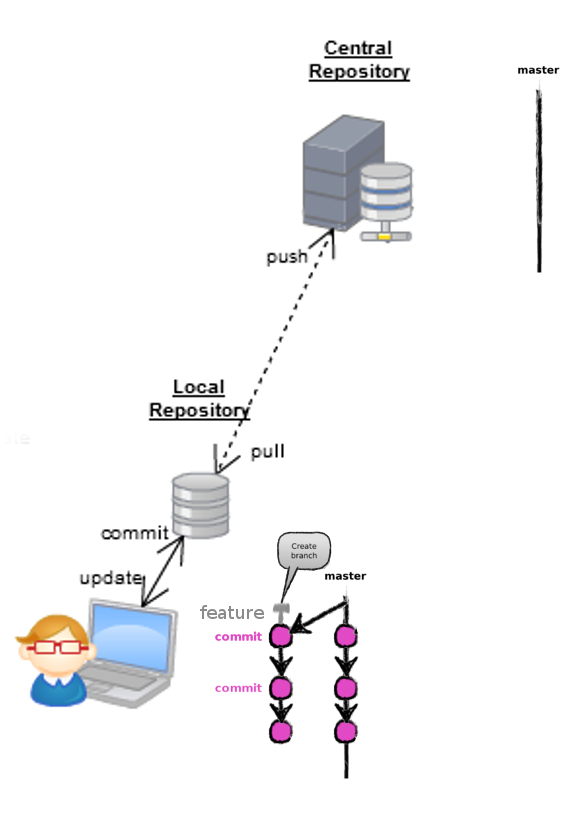
\includegraphics[width=0.9\textwidth]{branch_rebase.png}
			}\only<6> {
				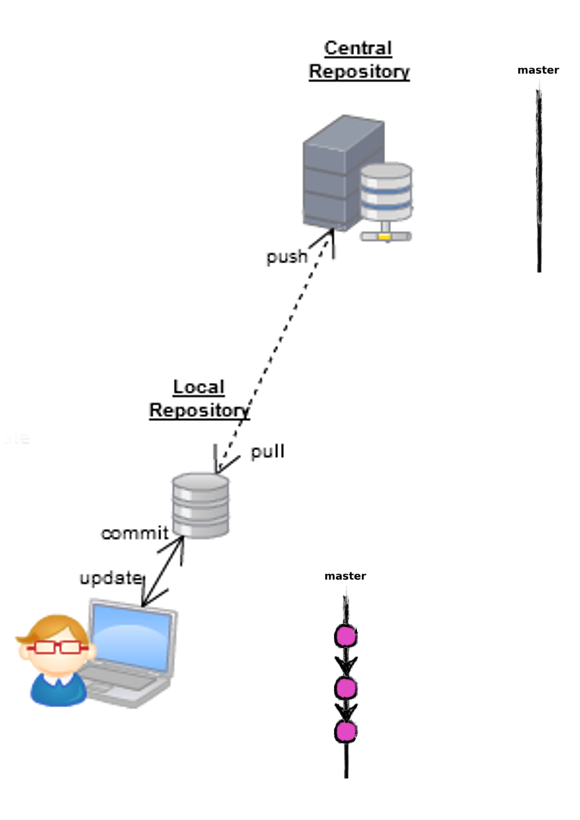
\includegraphics[width=0.9\textwidth]{branch_delete.png}
			}\only<7> {
				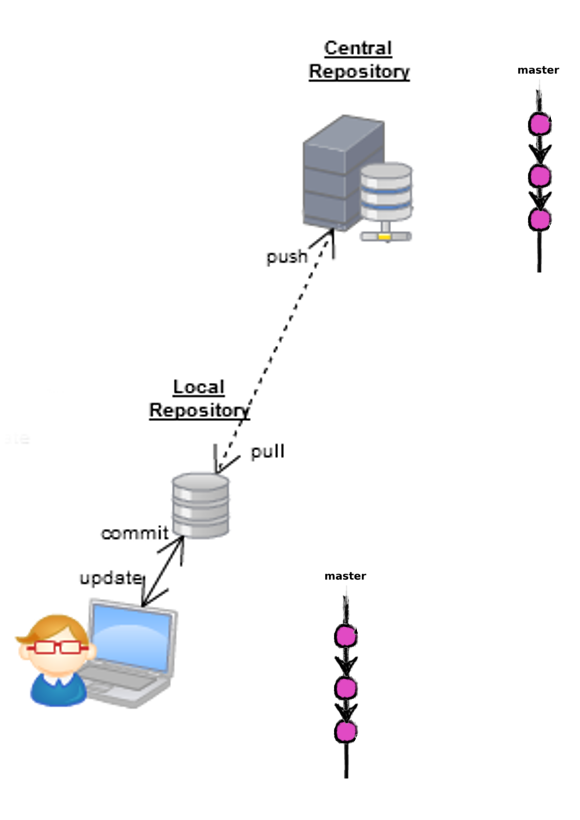
\includegraphics[width=0.9\textwidth]{branch_pushed.png}
			}\only<8> {
				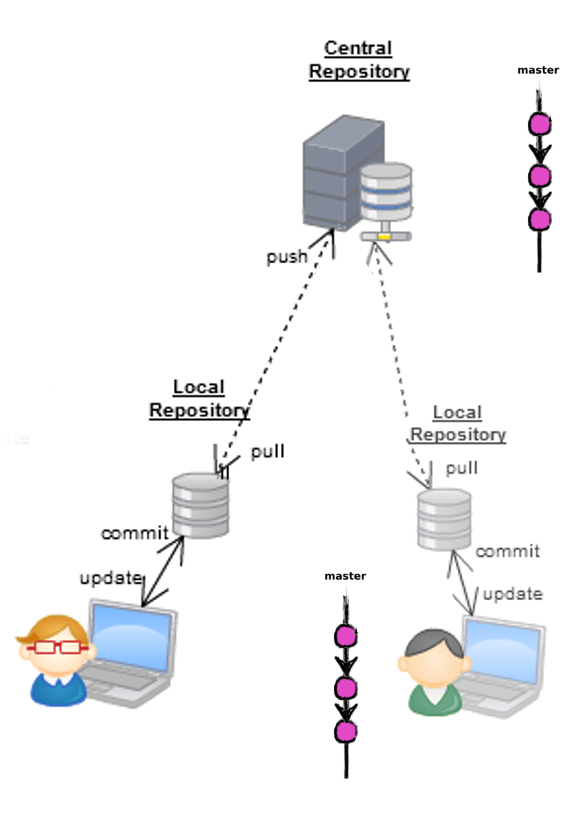
\includegraphics[width=0.9\textwidth]{branch_many.png}
			}
	\end{center}
\end{column}
\end{columns}

\visible<8>{
	\begin{center}
	
	\tiny
	\textit{What if I am not the only one working on this feature/bug?}
	\end{center}
}
\end{frame}

\setbeamercovered{transparent=0}

\begin{frame}[fragile]{Publish the branch on origin}
\begin{columns}
	\begin{column}{0.4\textwidth}
	\begin{lstlisting}
	|\pause|
$ # Push our branch 'feature' 
$ # to a new branch 'feature' 
$ # (will be created) on origin
$ git push origin feature:feature |\pause|

$ # From now on, to push (committed) changes...
$ git push origin feature
	\end{lstlisting}
	\end{column}
	\begin{column}{0.6\textwidth}
		\begin{center}
			\only<1> {
				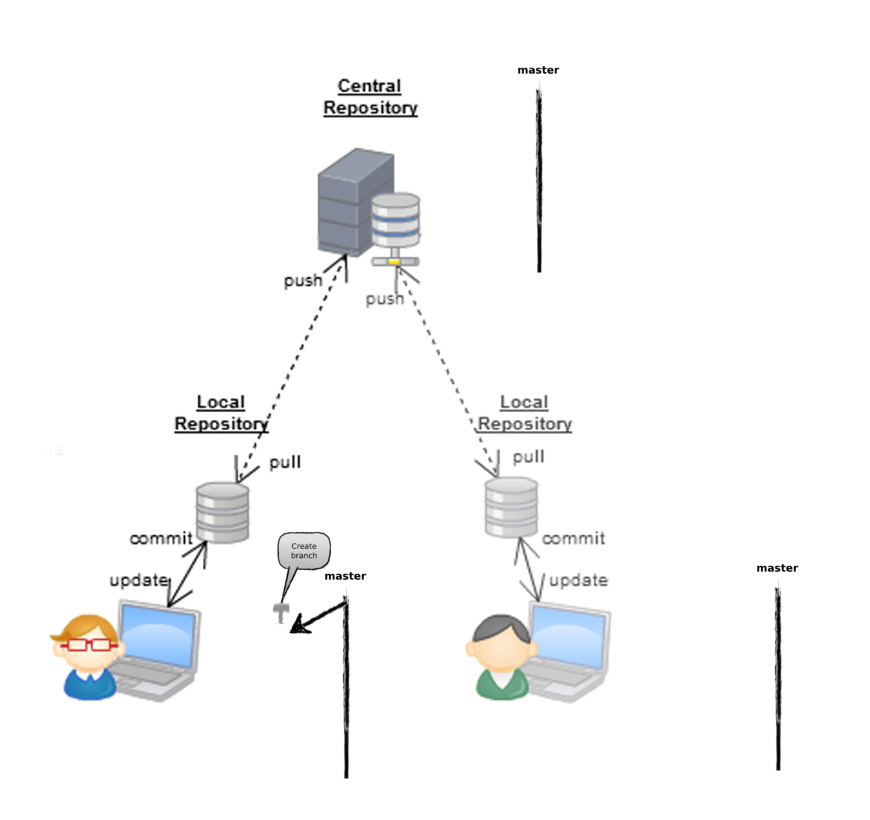
\includegraphics[width=.9\textwidth]{multiuser_local_branch.png}
			}\only<2> {
				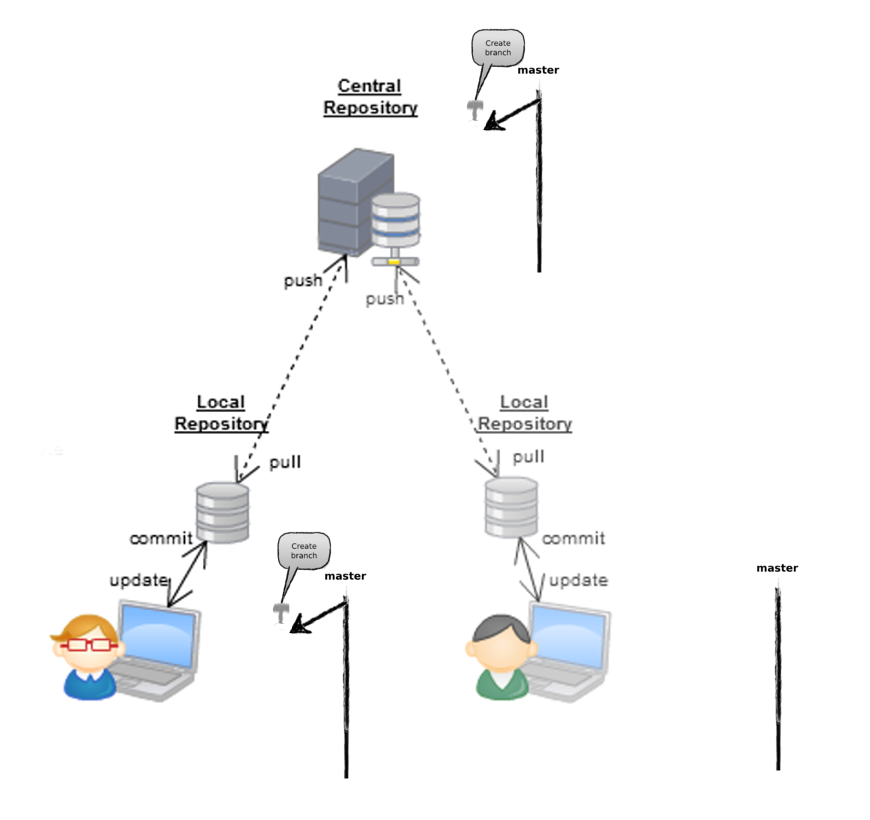
\includegraphics[width=.9\textwidth]{multiuser_remote_branch.png}
			}\only<3> {
				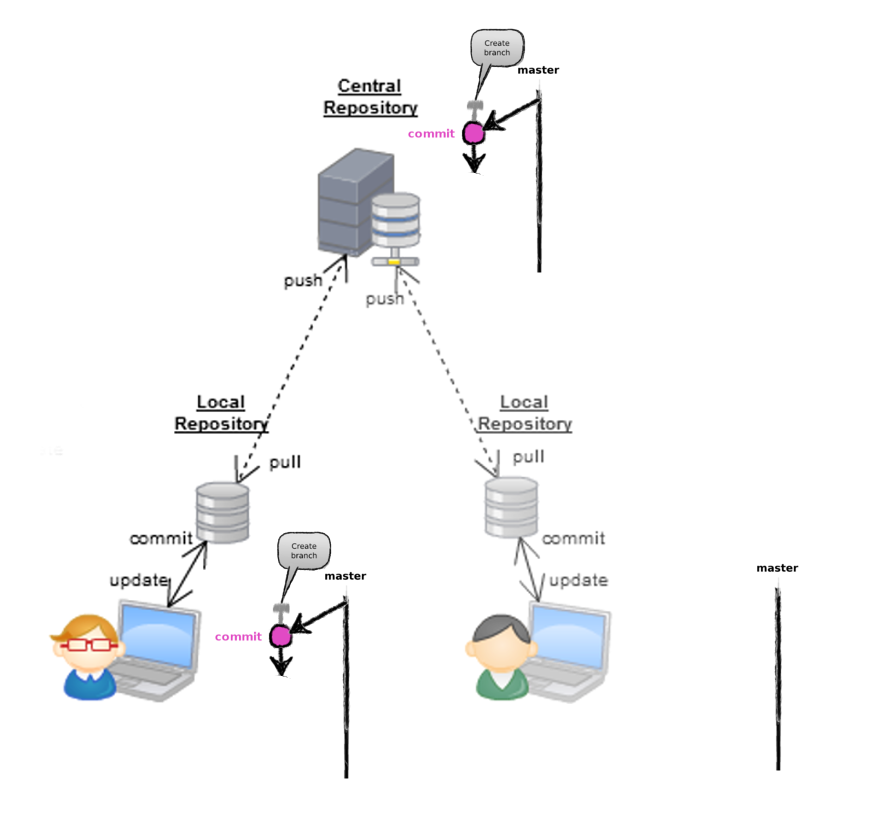
\includegraphics[width=.9\textwidth]{multiuser_push_branch.png}
			}
		\end{center}
	\end{column}
\end{columns}
\end{frame}


\begin{frame}[fragile]{Join someone else's branch}
\begin{columns}
	\begin{column}{0.4\textwidth}
	\begin{lstlisting}
$ git checkout --track -b feature origin/feature
Branch feature set up to track remote branch 
	refs/remotes/origin/feature.
Switched to a new branch "feature"
	\end{lstlisting}
	\visible<2->{
	\begin{tiny}
	{\color{eclipsePurple} Beware:} \textit{pull origin feature} would have merged the changes from the remote branch \textit{feature} into our current local branch!
	\end{tiny}
	}
	\end{column}
	\begin{column}{0.6\textwidth}
		\begin{center}
			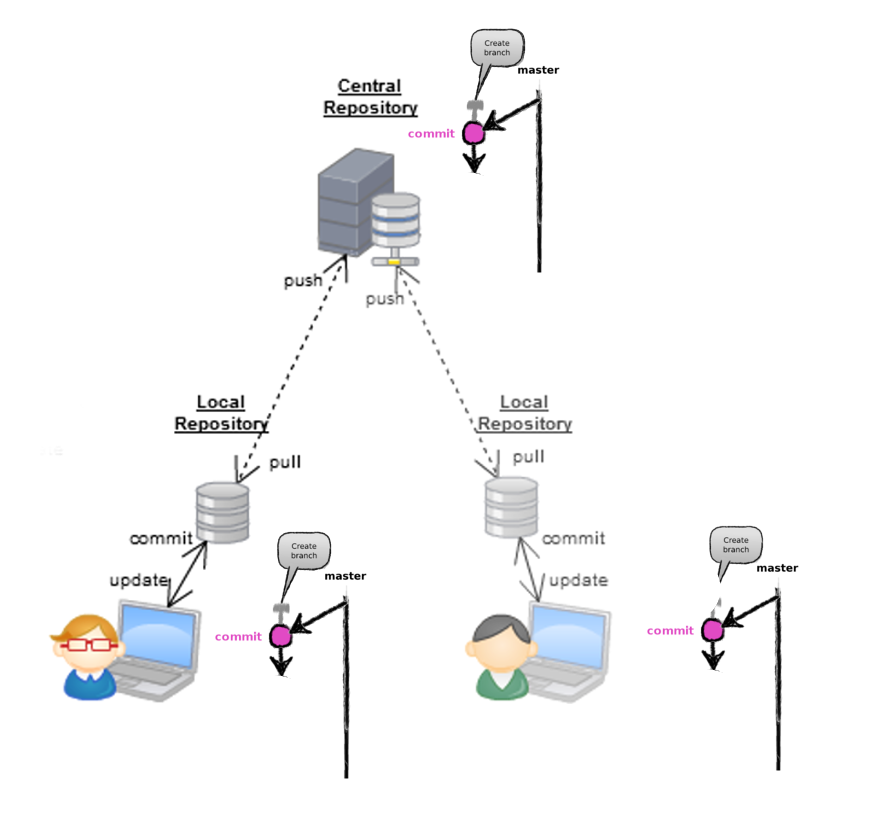
\includegraphics[width=.9\textwidth]{multiuser_track.png}
		\end{center}
	\end{column}
\end{columns}
\end{frame}


\begin{frame}[fragile]{Get updates from origin}
\begin{columns}
	\begin{column}{0.4\textwidth}
	\begin{lstlisting}
$ # Pull updates from origin
$ git pull |\pause|
     ...
There is no tracking information for the current branch.
Please specify which branch you want to merge with.
See git-pull(1) for details.

    git pull <remote> <branch> |\pause|
    
$ # Pull (from where?) from origin
$ # (what?) branch feature 
$ git pull origin feature |\pause|

$ # We can also update config...
$ # (from where?)
$ git config branch.feature.remote origin
$ # (what?)
$ git config branch.feature.merge feature

$ # ...so that from now on, 
$ # we can pull just by...
$ git pull
	\end{lstlisting}
	\end{column}
	\begin{column}{0.6\textwidth}
		\begin{center}
			\only<1-2> {
				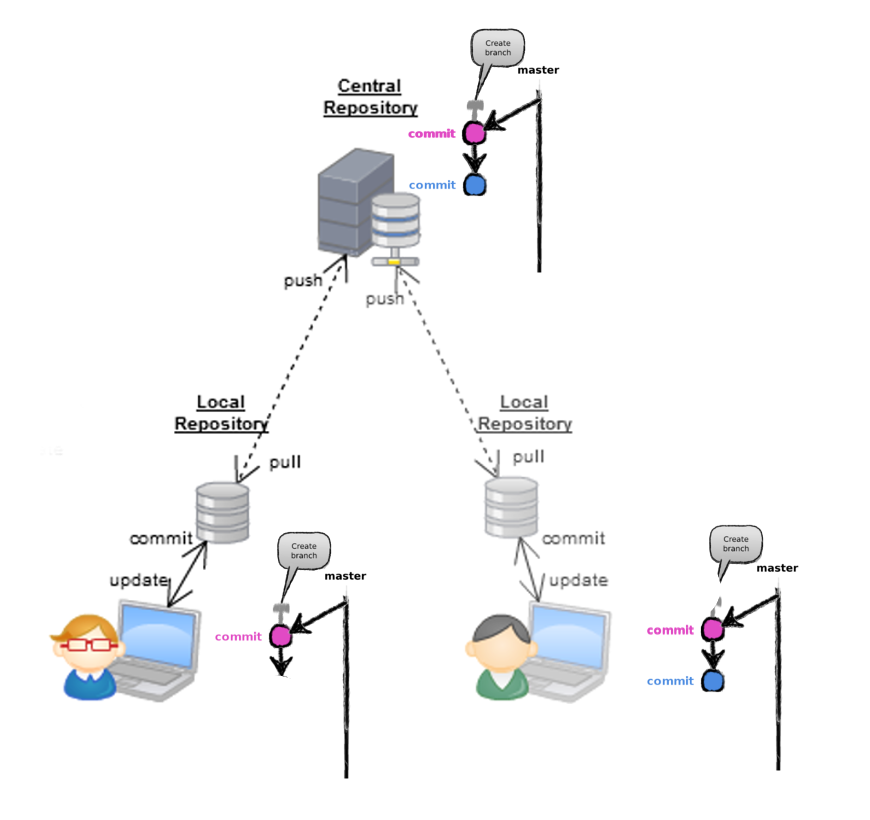
\includegraphics[width=.9\textwidth]{multiuser_they_push.png}
			}\only<3-> {
				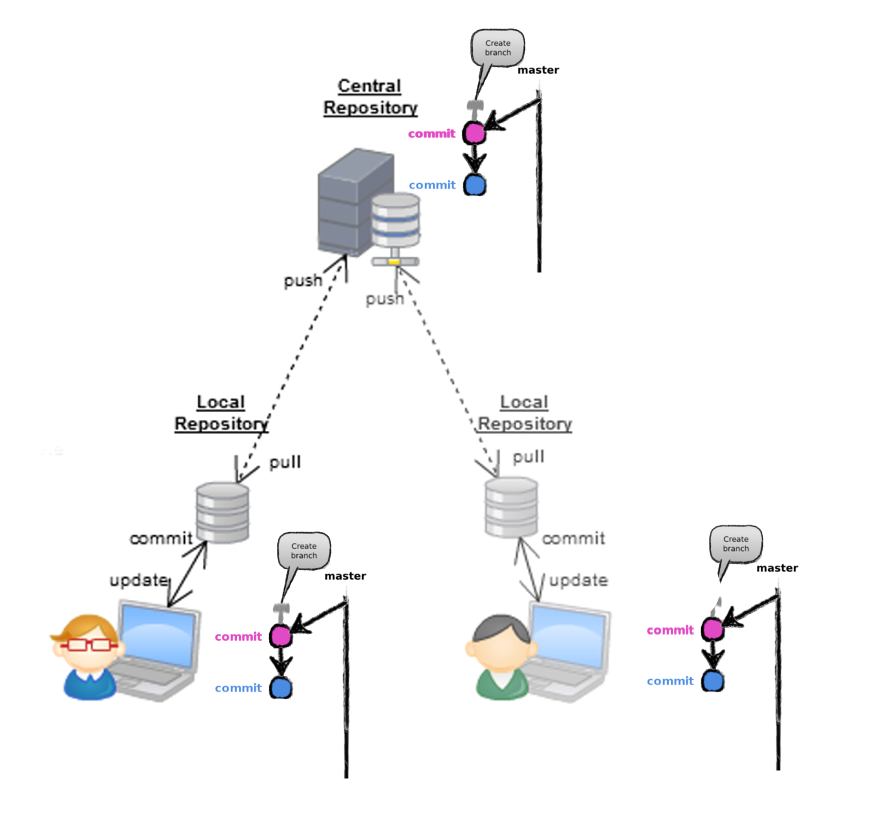
\includegraphics[width=.9\textwidth]{multiuser_pull.png}
			}
		\end{center}
	\end{column}
\end{columns}
\end{frame}


\begin{frame}[fragile]{Update the master}
\begin{columns}
	\begin{column}{0.4\textwidth}
  	\begin{lstlisting}
$ # Switch to master
$ git checkout master
Switched to branch "master" |\pause|

$ # Merge
$ git merge feature |\pause|

$ # Do not forget to push
$ git push
	\end{lstlisting}
	\end{column}
	\begin{column}{0.6\textwidth}
		\begin{center}
			\only<1> {
				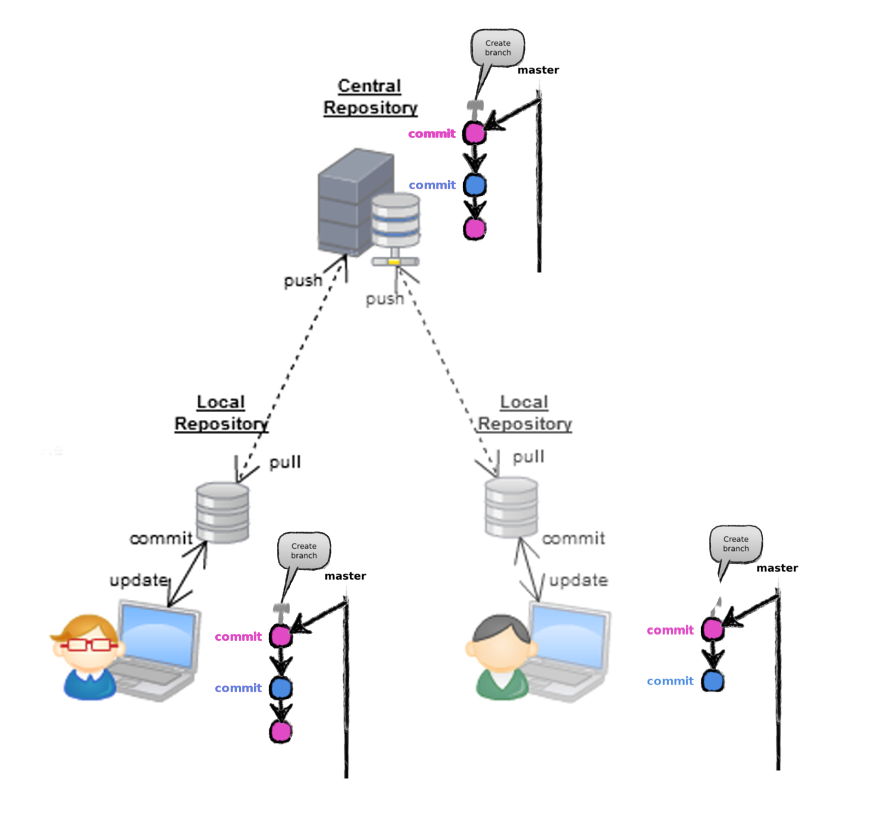
\includegraphics[width=.9\textwidth]{multiuser_my_many_commits_pushed.png}
			}\only<2> {
				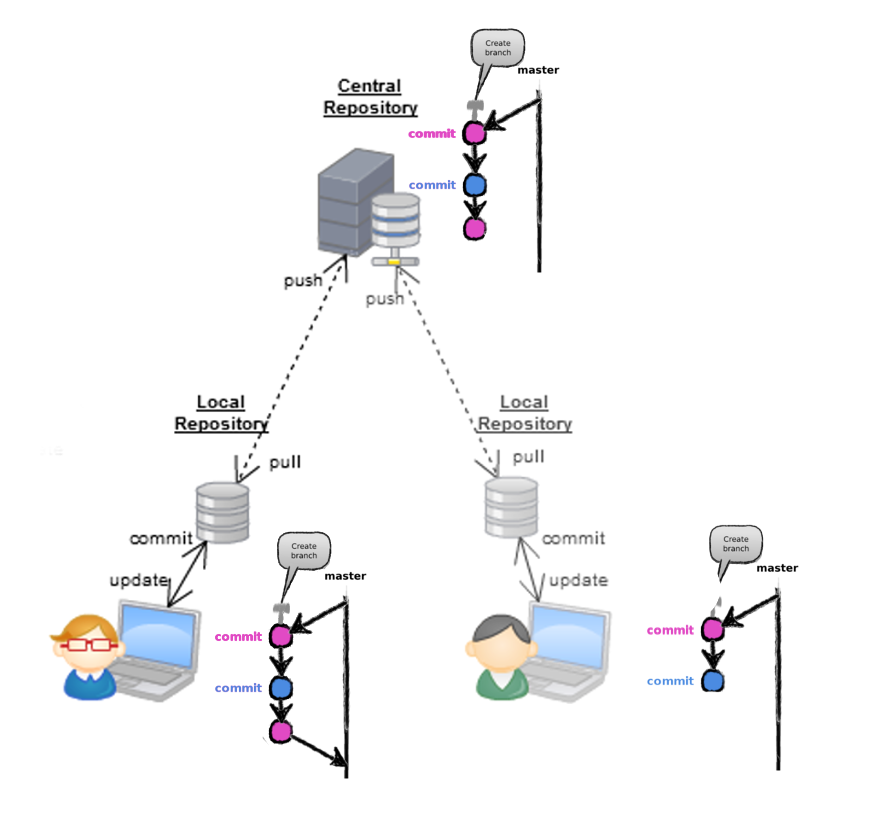
\includegraphics[width=.9\textwidth]{multiuser_my_merge.png}
			}\only<3-> {
				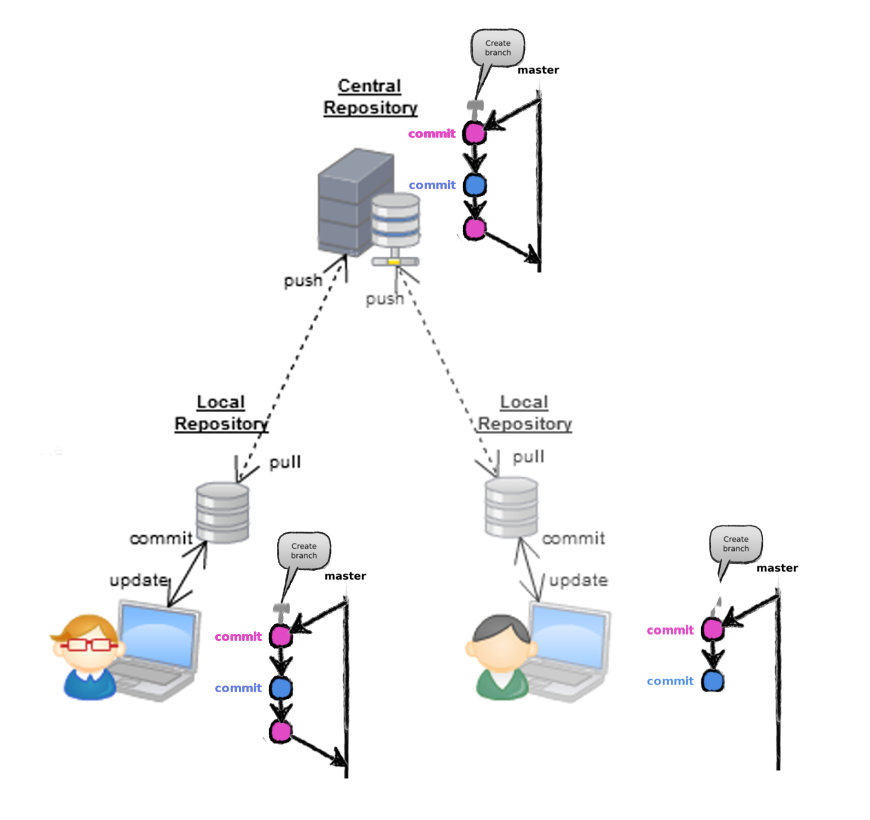
\includegraphics[width=.9\textwidth]{multiuser_remote_merge.png}
			}
		\end{center}
	\end{column}
\end{columns}
\end{frame}


\begin{frame}[fragile]{Remove the branch}
\begin{columns}
	\begin{column}{0.4\textwidth}
  	\begin{lstlisting}
$ # Remove local branch feature
$ git branch -d feature
Deleted branch feature (was fd86490). |\pause|


$ # Remove remote branch feature
$ git push origin :feature
- [deleted] feature
	\end{lstlisting}
	\end{column}
	\begin{column}{0.6\textwidth}
		\begin{center}
			\only<1> {
				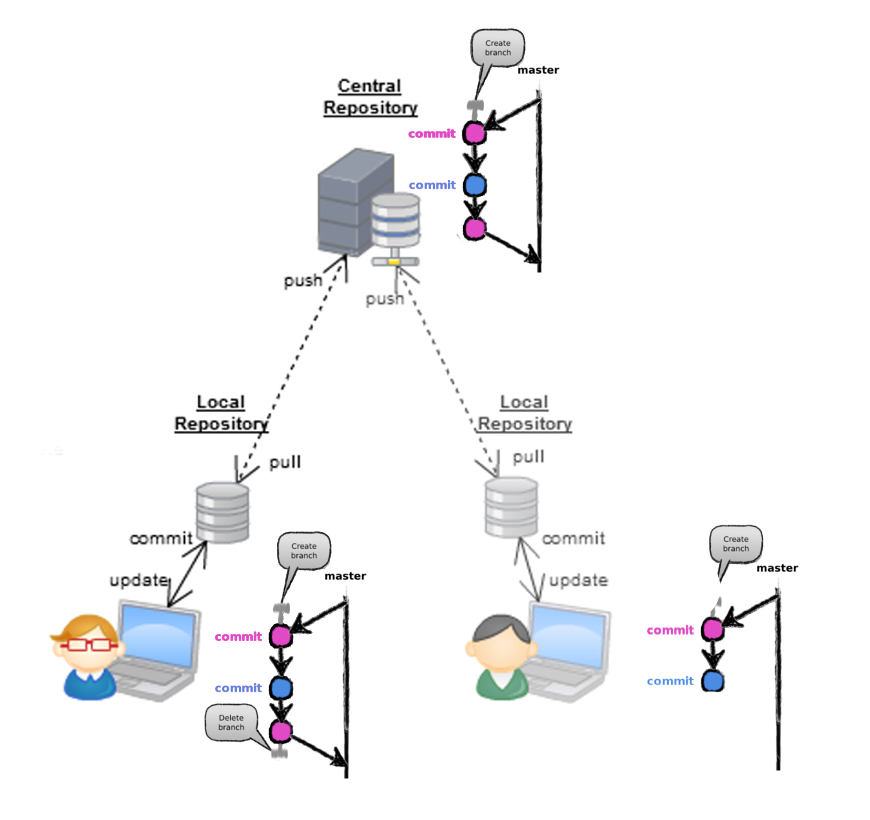
\includegraphics[width=.9\textwidth]{multiuser_my_delete.png}
			}\only<2> {
				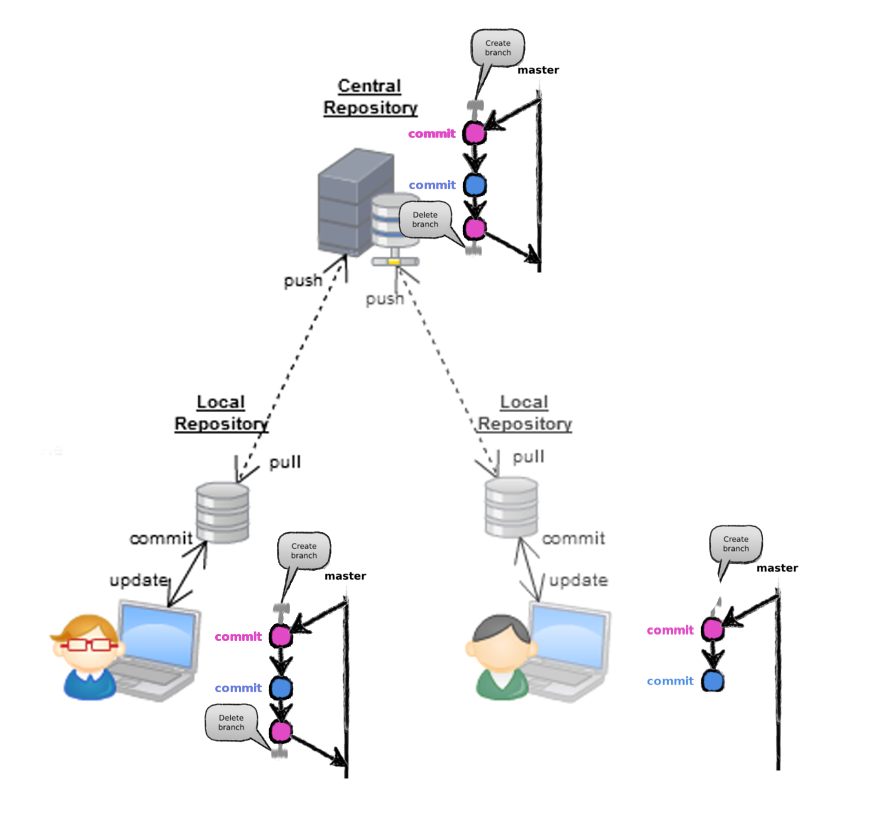
\includegraphics[width=.9\textwidth]{multiuser_remote_delete.png}
			}
		\end{center}
	\end{column}
\end{columns}
\end{frame}

\setbeamercovered{transparent=30}

\begin{frame}[fragile]{The scenario we've just seen}
\begin{columns}
\begin{column}{0.5\textwidth}
	\tiny
	\begin{enumerate}
		\item<1-2> Created a new branch locally \\\textbf{and published it on the remote origin}
		\item<3-4> Implemented a new feature/Fixed a bug
		\begin{enumerate}
			\tiny
			\item<3> Step 1 towards new feature/bug fix
			\item<3> Commit \textbf{(and maybe push to origin)}
			\item<3> \ldots
			\item<4> \textbf{Pull others' changes from origin}
			\item<4> \ldots
		\end{enumerate}
		\item<5> \textbf{Merged} this branch with the master \textbf{locally}
		\item<6> \textbf{Pushed changes to origin}
		\item<7-> Deleted this branch locally \textbf{and on origin}
	\end{enumerate}
\end{column}
\begin{column}{0.6\textwidth}
	\begin{center}
			\only<1> {
				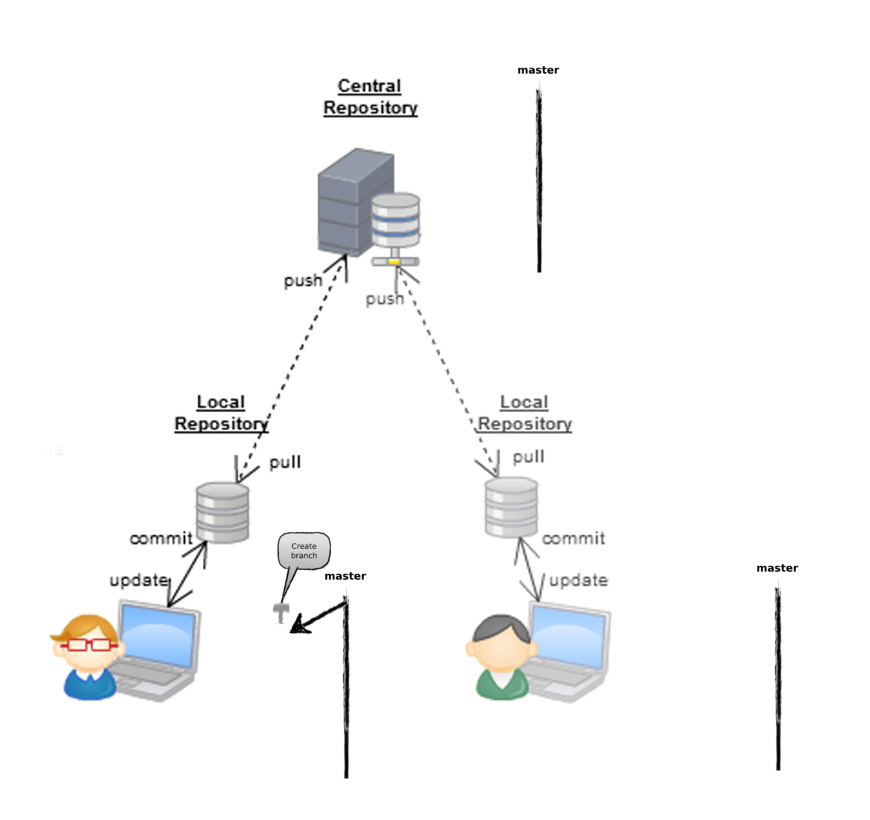
\includegraphics[width=0.9\textwidth]{multiuser_local_branch}
			}\only<2> {
				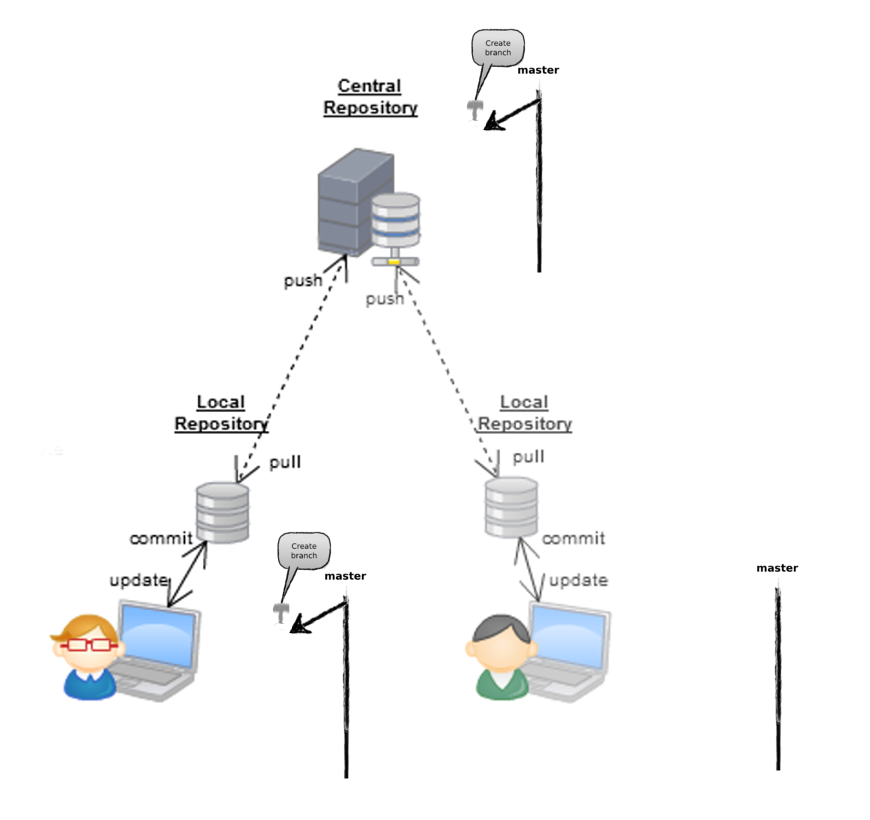
\includegraphics[width=0.9\textwidth]{multiuser_remote_branch}
			}\only<3> {
				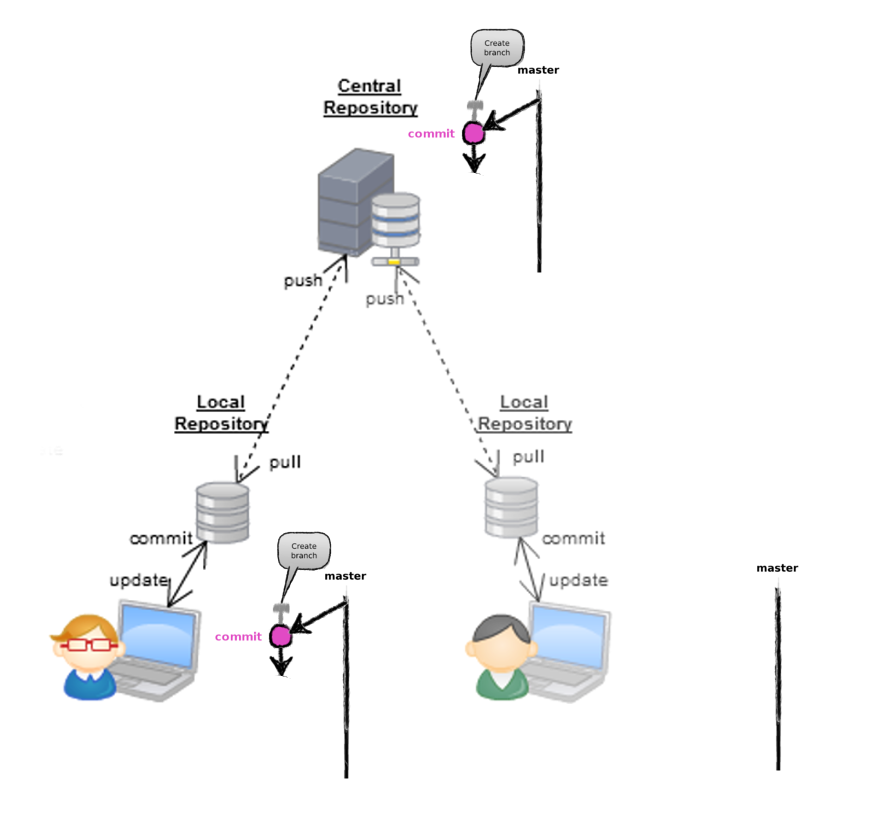
\includegraphics[width=0.9\textwidth]{multiuser_push_branch}
			}\only<4> {
				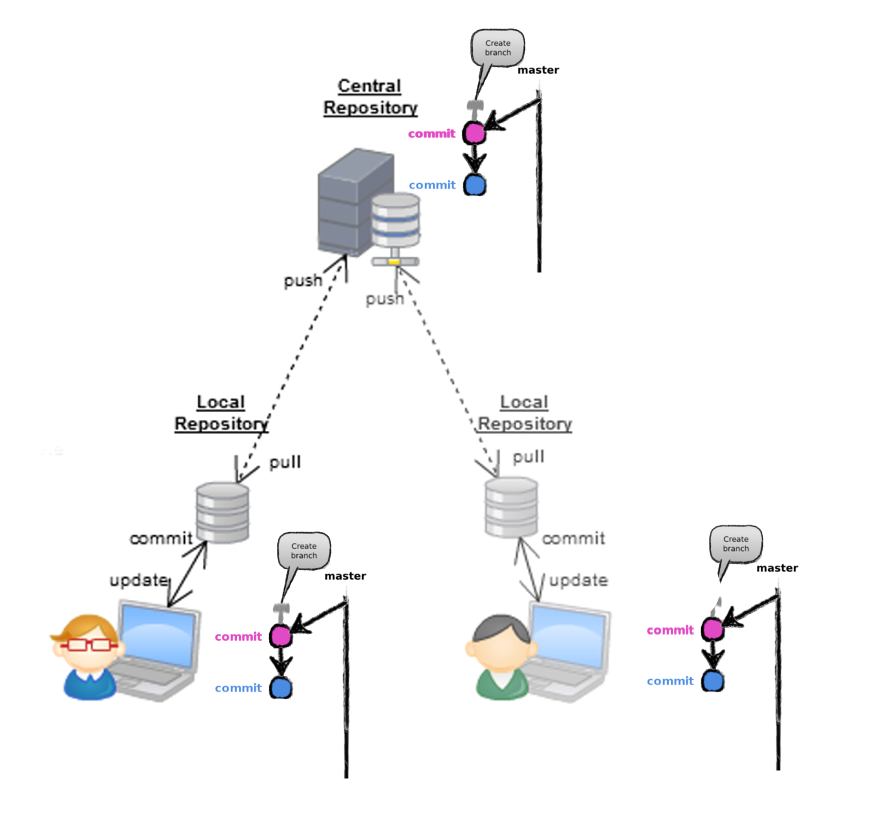
\includegraphics[width=0.9\textwidth]{multiuser_pull.png}
			}\only<5> {
				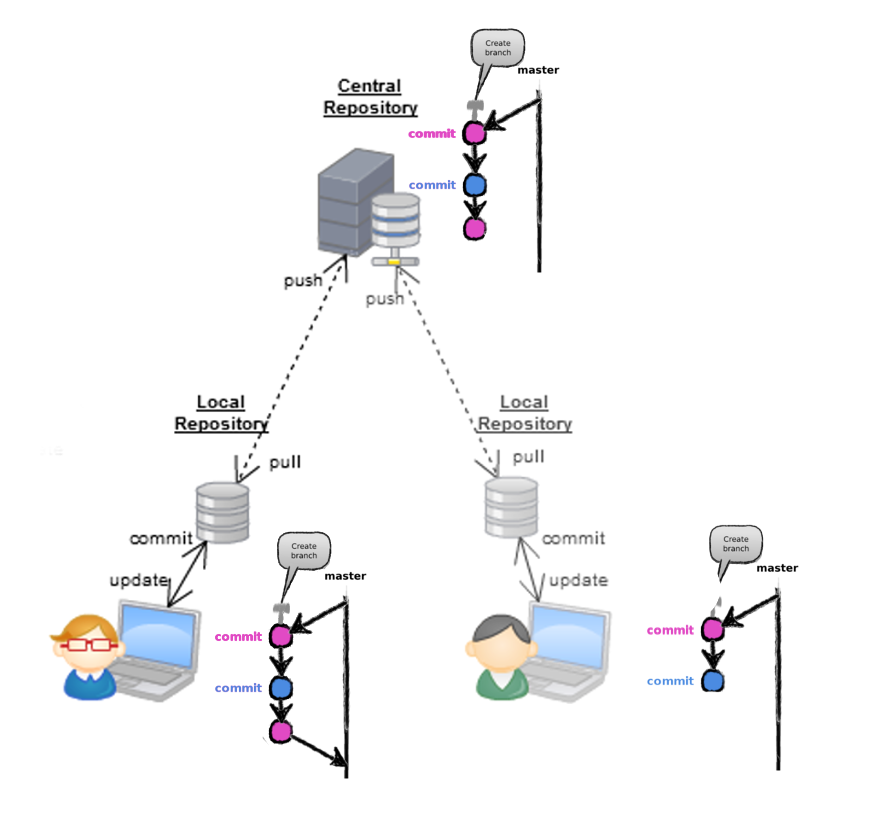
\includegraphics[width=0.9\textwidth]{multiuser_my_merge.png}
			}\only<6> {
				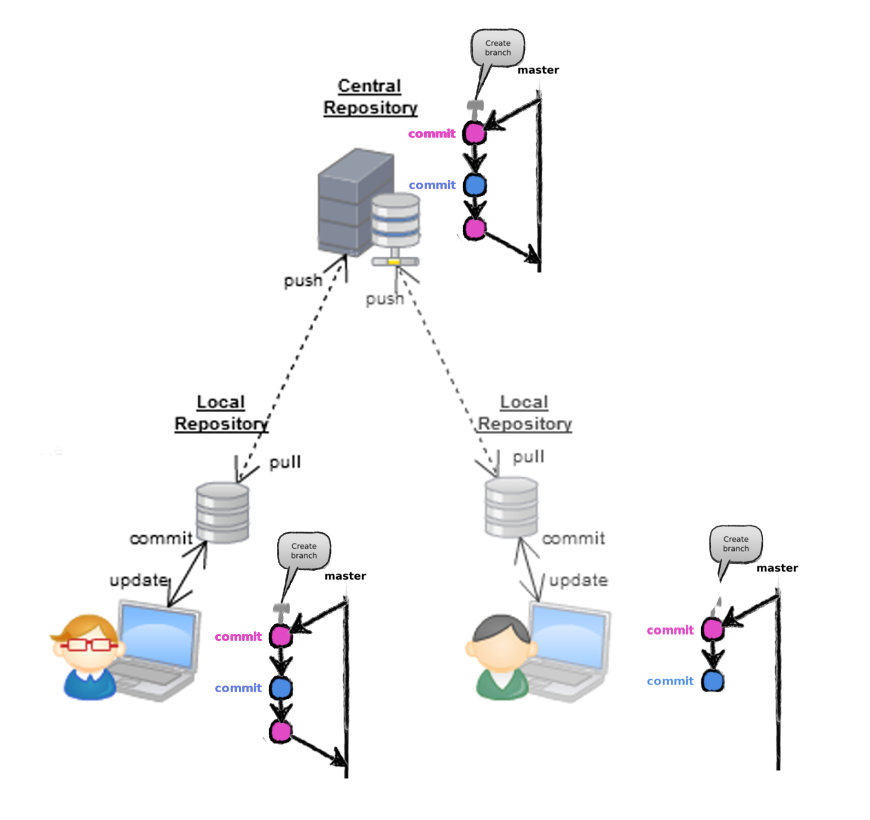
\includegraphics[width=0.9\textwidth]{multiuser_remote_merge.png}
			}\only<7> {
				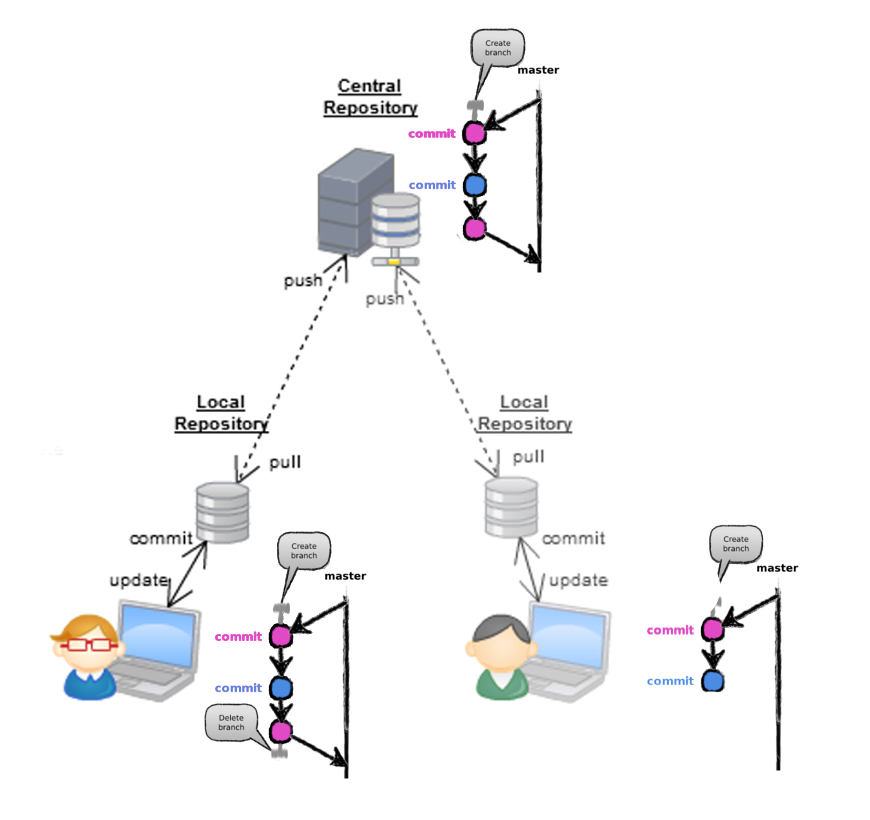
\includegraphics[width=0.9\textwidth]{multiuser_my_delete.png}
			}\only<8> {
				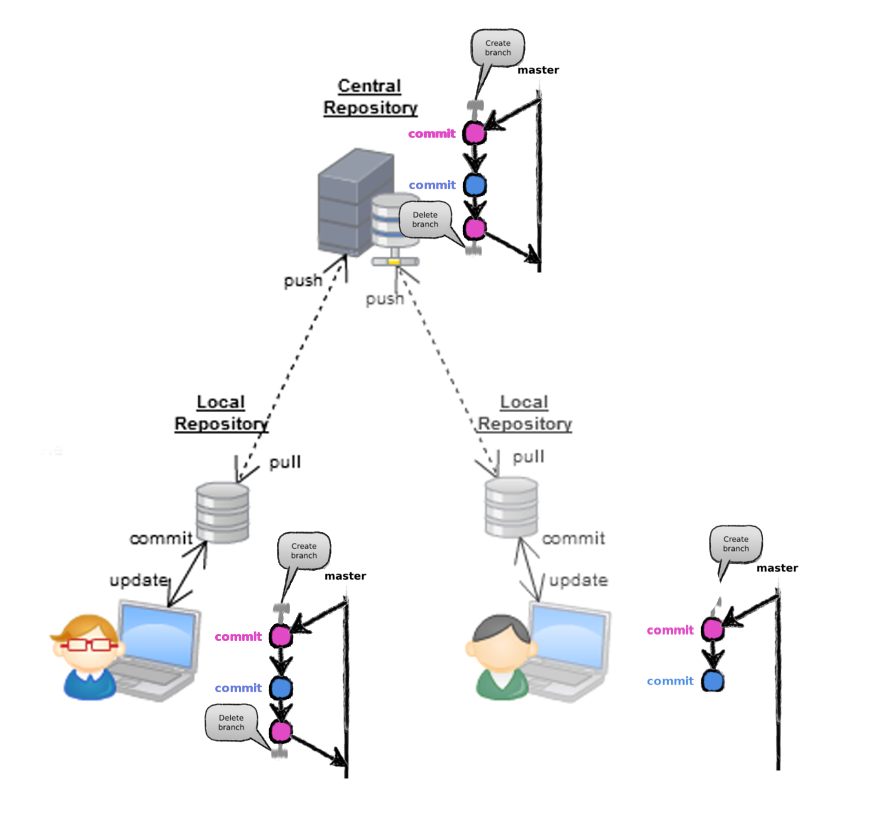
\includegraphics[width=0.9\textwidth]{multiuser_remote_delete.png}
			}
	\end{center}
\end{column}
\end{columns}
%	\pause
%	\textit{What if I want to work in several branches in parallel?}
\end{frame}


\begin{frame}{Summary}
	\begin{tiny}
    \begin{itemize}
        \item[] {\color{eclipseBlue}git init} -- create an empty repository
        \item[] {\color{eclipseBlue}git clone <repository>} -- clone a repository into a new directory
        \item[]
        \item[] {\color{eclipseBlue}git branch -a} -- list existing branches
        \item[] {\color{eclipseBlue}git branch <branch>} -- create a branch
        \item[] {\color{eclipseBlue}git checkout <branch>} -- switch to the branch 
        \item[]
        \item[] {\color{eclipseBlue}git status} -- show the working tree status
        \item[] {\color{eclipseBlue}git add <filepath>} -- add a file to the index (to be committed)
        \item[] {\color{eclipseBlue}git commit -m <message>} -- record changes to the local repository
        \item[]
        \item[] {\color{eclipseBlue}git pull <from where?> <which branch?>} -- fetch and integrate changes
        \item[] {\color{eclipseBlue}git push <where?> <to which branch?>} -- push the changes the remote repository
        \item[]
        \item[] {\color{eclipseBlue}git merge <branch>} -- merge the selected branch into the current branch
        \item[] {\color{eclipseBlue}git rebase <branch>} -- reapply commits from the branch on top of the current branch
%        \item[]
%        \item[] {\color{eclipseBlue}git stash} -- record the current state of the working directory and the index, and clean the working directory
%        \item[] {\color{eclipseBlue}git stash list} -- list the stashes that currently exist
%        \item[] {\color{eclipseBlue}git stash apply <stash>} -- return to the state recorded in this stash
        \item[]
        \item[] {\color{eclipseBlue}git log [-{}-graph]} -- see commit logs
        \item[]
        \item[] {\color{eclipseBlue}git config [-{}-global] <key> <value>} -- set config option
    \end{itemize}
    
    \begin{center}
    	Detailed docs: \url{https://git-scm.com/docs}
    \end{center}
    \end{tiny}
\end{frame}


\section{Hosting services}
% List hosting services and what they add
\definecolor{git}{RGB}{172, 49, 49}
\def\git#1{{\small\color{git}\$ git #1}\\}

\begin{frame}[fragile]{Why not just local git?}
  \begin{itemize}
  \item<1-> Local git alone via command line: Ok
  \item<2-> But lack of functionalities:
    \begin{itemize}
    \item User/permission management
    \item Bug tracking
    \item Duscussing implementations
    \item Forking other projects
    \item Easy collaborative development 
    \end{itemize}
  \item<3-> Several services were developed around git
    \begin{itemize}
    \item 
\includegraphics[width=15px]{images/GitHub-Mark.png} GitHub \url{https://github.com/}
    \item 
\includegraphics[width=15px]{images/bitbucket.png} bitbucket \url{https://bitbucket.org/}
    \item 
\includegraphics[width=15px]{images/GitLab_Logo.png} GitLab \url{https://git.framasoft.org/}
    \item ...
    \end{itemize}
  \end{itemize}
\end{frame}

\begin{frame}{GitHub}
  \begin{itemize}
  \item url : https://GitHub.com/ 
  \item Wikipedia: GitHub is a web-based Git repository hosting service. It offers all of the distributed revision control and source code management (SCM) functionality of Git as well as adding its own features. Unlike Git, which is strictly a command-line tool, GitHub provides a Web-based graphical interface and desktop as well as mobile integration. It also provides access control and several collaboration features such as bug tracking, feature requests, task management, and wikis for every project.
  \end{itemize}
\end{frame}



\section{Practical work}
% hands on 
%

% For the teachers: create a repo 
% create a branch called dev.



 
\begin{frame}{Requirement}
    \begin{enumerate}
        \item Install git
        \item Set up your git config
        \item Create an account on github
        \item Set up your ssh-key
    \end{enumerate}
\end{frame}

\begin{frame}{Practical work 1}
    \begin{enumerate}
        \item Clone https://github.com/C3BI-pasteur-fr/sandbox
        \item Create a file. Put your name for the filename
        \item Push this file on the repository (add, commit, push)
    \end{enumerate}
    \begin{alertblock}<2>{Problem}
        Every one try to add his file on the master.
    \end{alertblock}
\end{frame}




\section{Advanced git}
% More advanced usage
\begin{frame}[fragile]{Working in several branches in parallel}
	\begin{tiny}
		\begin{lstlisting}
$ # On branch A: did some changes, but not yet ready to commit...
$ # Want to switch to branch B. |\pause| Checkout?
$ git checkout master
error: Your local changes to the following files would be overwritten by checkout:
	main/basic_git.tex
Please, commit your changes or stash them before you can switch branches.
Aborting |\pause|

$ # Save the changes first.
$ git stash
Saved working directory and index state WIP on basic_git: 30fb6e8 Fixed typos
HEAD is now at 30fb6e8 Fixed typos |\pause|

$ # Now we can switch to another branch and work there...
$ git checkout master
Switched to branch 'master'
$ ...
		\end{lstlisting}
	\end{tiny}
\end{frame}

\begin{frame}[fragile]{Working in several branches in parallel}
	\begin{tiny}
		\begin{lstlisting}
$ # Back on branch A: How do I get my changes back?
$ # Which stashes are there?
$ git stash list
stash@{0}: WIP on master: ceef0bd Merge pull request #1 from C3BI-pasteur-fr/services
stash@{1}: WIP on basic_git: 30fb6e8 Fixed typos |\pause|

$ # Apply the stash
$ git stash apply stash@{1}
On branch basic_git
Changes not staged for commit:
  (use "git add <file>..." to update what will be committed)
  (use "git checkout -- <file>..." to discard changes in working directory)

	modified:   basic_git.tex
	... |\pause|
	
$ # Remove this stash from stash list
$ git stash drop stash@{1}
Dropped stash@{1} (739c015cafdc37e22a45d97868c3d03bc940eadf)
		\end{lstlisting}
	\end{tiny}
\end{frame}

\end{document}
